\chapter{Background}
\label{ch:object-detection}
\section{Fundamentals of Object Detection}
% What's object detection? Describe the task itself, how it differs from  classification and other computer vision tasks. What are the usual approaches in the deep learning context (one-stage vs two-stage, anchor-based vs anchor-free, etc.)? What are the most common architectures and their characteristics? 
% highlight problems related to their structured outputs and the inherited challenges for gradient backpropagation 

Object detection is one of the fundamental task in computer vision that involves localizing and classifying multiple objects within an image. Unlike image classification and other tasks that assign a single label to an individual image, object detection requires predicting a set of bounding boxes, each associated with a class label and a confidence score. The challenging nature of this output stems from the variable cardinality of such sets, as the number of objects in an image can vary significantly, leading to complex structured prediction problems.

To address these challenges in a principled manner, it is useful to describe object detection as a structured prediction problem. This framework not only clarifies the task requirements but also provides a common language for comparing different detection architectures and loss functions.\\

Let an image be denoted as 
$
x \in \mathbb{R}^{H \times W \times C},
$
where $H$ and $W$ are the spatial dimensions and $C$ is the number of channels.
The output of an object detector is a finite set of detections:
$$
\mathcal{D} = \{ (b_i, y_i, s_i) \}_{i=1}^N,
$$
where:
\begin{itemize}
    \item $b_i = (x_i, y_i, w_i, h_i)$ represents the bounding box in pixel coordinates in COCO format (center position, width, height);
    \item $y_i \in \{1, \dots, K\}$ is the predicted class label, with $K$ the total number of object classes;
    \item $s_i \in [0,1]$ is the confidence score, often interpreted as the estimated probability that $b_i$ belongs to class $y_i$.
\end{itemize}

During training, ground-truth bounding boxes $b_i^\ast$ are typically transformed into target regression parameters relative to reference boxes (anchors or proposals) as:
$$
t_x = \frac{x^\ast - x_a}{w_a}, \quad
t_y = \frac{y^\ast - y_a}{h_a}, \quad
t_w = \log \frac{w^\ast}{w_a}, \quad
t_h = \log \frac{h^\ast}{h_a},
$$
where $(x_a, y_a, w_a, h_a)$ are the anchor box parameters, and $(x^\ast, y^\ast, w^\ast, h^\ast)$ are the corresponding ground-truth parameters.

The specific optimization objectives used for bounding box regression and classification are detailed in Section~\ref{sec:loss_functions}, following the description of the detection architectures.

The object detection task can thus be formalized as learning a function:
$$
f_\theta: \mathbb{R}^{H \times W \times C} \to \mathcal{P}(\mathbb{R}^4 \times \{1, \dots, K\} \times [0,1]),
$$
parameterized by $\theta$, that maps an input image to a set of bounding box--label--score triples.
The set-valued nature of $\mathcal{P}(\cdot)$ reflects that the number of detections varies between images.

This formalization underpins the taxonomy of detection architectures discussed in the following section, where we distinguish between one-stage and two-stage approaches, anchor-based and anchor-free formulations, and their respective training and inference paradigms.

\subsubsection{Feature Pyramid Networks (FPN)}
Before diving into the specific architectures, we introduce a widely used component in most object detection models: the Feature Pyramid Network (FPN).

Objects appear at widely varying scales, early CNN backbone layers produce high-resolution but semantically weak features (shallow layers), while deeper layers produce low-resolution but semantically strong features.
FPNs fuse these to obtain semantically strong, multi-scale feature maps at multiple resolutions, enabling detectors to handle small and large objects efficiently with a single backbone pass (as opposed to costly image pyramids)~\cite{lin2017fpn}.\\

Let $\{C_2,C_3,C_4,C_5\}$ be backbone feature maps with strides $\{4,8,16,32\}$ w.r.t.\ the input.
FPN builds $\{P_2,P_3,P_4,P_5\}$ by a top–down pathway and lateral merges as shown in Figure~\ref{fig:fpn-lateral}.

\begin{figure}[h]
    \centering
    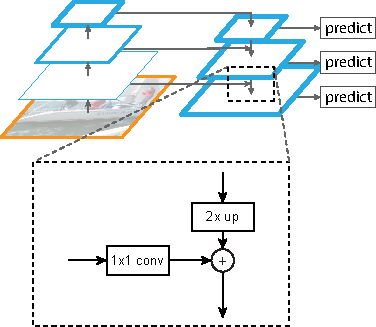
\includegraphics[]{images/fpn-lateral.pdf}
    \caption{A building block illustrating the lateral connection and
    the top-down pathway, merged by addition \cite{lin2017fpn}}
    \label{fig:fpn-lateral}
\end{figure}


\subsection{One-Stage vs Two-Stage Detectors}

Object detectors can be broadly categorized into \emph{one-stage} and \emph{two-stage} paradigms. Both ultimately predict a variable-sized set of detections $\mathcal{D} = \{(b_i, y_i, s_i)\}$, but they differ in how they structure intermediate computations and where they allocate capacity for localization vs.\ classification.

\subsubsection{Two-stage detectors.}
Two-stage methods decompose detection into proposal generation followed by proposal classification and box refinement. Let $g_{\phi}$ denote a proposal mechanism (e.g., a region proposal network operating on a shared backbone), which maps an image $x$ to a set of candidate regions $\mathcal{P}$:
$$
\mathcal{P} = g_{\phi}(x) = \{p_j\}_{j=1}^{M}.
$$
A second function $f_{\theta}$ then classifies and refines these regions to produce final detections:
$$
\mathcal{D} = f_{\theta}(x, \mathcal{P}).
$$
Operationally, the pipeline is:
\begin{enumerate}
    \item Backbone (optionally with a feature pyramid) extracts multi-scale features from $x$.
    \item A proposal generator produces a sparse set of regions $\mathcal{P}$ (typically with non-maximum suppression to reduce redundancy).
    \item Per-region features are pooled/aligned from the shared feature maps and passed to a detection head to output class scores and refined boxes.
\end{enumerate}

The idea underlying two-stage detectors is to incentivise accuracy by first generating a manageable number of promising candidates, which can then be processed and refined with more complex per-region heads. This also allows for a more efficient use of computational resources, as the second stage can focus on a smaller set of regions rather than processing the entire image densely.
But unfortunately, this approach introduces a fair amount of complexity requiring careful design.

\subsubsection{One-stage detectors.}
One-stage methods simplify the detection pipeline by predicting detections directly from the shared feature maps without an explicit proposal stage. This design is motivated by the desire to maximize throughput and reduce latency, particularly in real-time applications. This type of detection is often referred to as \emph{dense predictions} because it involves predicting detections at every spatial location of the feature maps, often having to take into account hundreds of thousands of locations per image.
Conceptually, it implements a direct mapping
$$
\mathcal{D} = h_{\psi}(x),
$$
where $h_{\psi}$ produces, for each spatial location (and possibly for multiple predefined reference shapes), joint classification scores and box parameters. The pipeline is:
\begin{enumerate}
    \item Backbone (optionally with a feature pyramid) extracts multi-scale features from $x$.
    \item Lightweight prediction heads applied densely over feature maps output $(b, y, s)$ candidates.
    \item A single-stage post-processing (e.g., top-$k$ filtering and non-maximum suppression) yields $\mathcal{D}$.
\end{enumerate}
This design maximizes throughput and simplifies the graph, but operates under severe class imbalance, due to the fact that most locations tend to be related to a generic background class, and thus the model has to learn to distinguish between a very large number of background locations and a comparatively small number of foreground locations. This imbalance is often addressed with specialized loss functions, such as the Focal Loss \cite{lin2018focalloss}, which down-weights easy-to-classify examples and focuses training on hard negatives.
The precision of the predictions often relies on effective assignment and post-processing techniques.
An alternative way of addressing this imbalance, ironically, is to use a two-stage approach, where the first stage takes care of separating the foreground (potential candidates) from the background.

\paragraph{Comparative characteristics.}
One might ask "Which paradigm is better then?" and the answer would be, as usual, "it depends". One-stage detectors are generally faster and more resource-efficient, and that is because they were intended to address the latency and throughput requirements of real-time applications. This comes at the cost of some accuracy that two-stage detectors can achieve with their more careful filtering mechanisms and (usually) more complex per-region heads that come at the cost of increased compatuational requirements and latency. And similarly one-stage detectors, they were designed to be accurate rather than fast.

Ideally one would like to have the best of both worlds, and we can find in literature a number of approaches that tries to reach two-stage performance with one-stage efficiency, such as the RetinaNet and YOLO \cite{lin2018focalloss,redmon2016yolo}.

We can summarize the main differences between one-stage and two-stage detectors as follows:
\begin{itemize}
    \item \textbf{Computation.} Two-stage: cost scales with the number of proposals $M$ (feature pooling and per-RoI head). One-stage: cost scales with the number of feature locations (and reference shapes) processed densely.
    \item \textbf{Capacity allocation.} Two-stage allocates more parameters per candidate via the second-stage head; one-stage relies on shallow, shared heads and benefits from strong multi-scale features.
    \item \textbf{Class imbalance.} One-stage training observes extreme foreground/background imbalance due to dense supervision; two-stage partially mitigates this by filtering with proposals and sampling strategies.
    \item \textbf{Latency/throughput.} One-stage typically achieves lower latency and higher FPS; two-stage often offers higher accuracy at increased computational cost.
    \item \textbf{Post-processing.} Two-stage commonly applies suppression both after proposal generation and after final classification; one-stage applies it once on dense predictions (often per class).
\end{itemize}


% \paragraph{Outlook.}
% In what follows, we instantiate these paradigms with canonical representatives: a one-stage detector with dense predictions, and a two-stage detector with proposals followed by RoI-level classification and refinement, both using feature pyramids to extract multi-scale features. We subsequently discuss anchor-based vs.\ anchor-free formulations, which apply orthogonally to both paradigms.


\subsection{Anchor-Based vs.\ Anchor-Free}

Object detectors differ not only by staging (one- vs.\ two-stage) but also by how they parameterize candidate boxes. The two prevailing choices are \emph{anchor-based} (predefined reference boxes) and \emph{anchor-free} (direct box prediction without references). This design is largely orthogonal to the staging paradigm.

\subsubsection{Anchor-based detectors}
\label{sec:anchor_based_detectors}
Let $\mathcal{A}=\{a_k\}_{k=1}^{K}$ be a set of predefined anchors tiled over feature maps. 
Each anchor $a_k=(x_a,y_a,w_a,h_a)$ serves as a reference against which a detector predicts offsets $(t_x,t_y,t_w,t_h)$ to obtain a box:
$$
x = x_a + w_a t_x \quad
y = y_a + h_a t_y \quad
w = w_a e^{t_w} \quad
h = h_a e^{t_h}
$$

Anchors are generated at multiple scales and aspect ratios per spatial location and per FPN level $\ell$ (with stride $s_\ell$), e.g.\ scales $\{s_\ell \cdot \alpha\}$ and ratios $r \in \{1\!:\!2,\,1\!:\!1,\,2\!:\!1\}$.
The number of anchors generated for each image tends to be large, but since we're considering the spatial locations of the feature maps, and not the original image, this number is still manageable, although it can still be in the order of hundreds of thousands, depending on the number of feature maps, stride, number of scales, aspect ratios and size of the image.\\

Training uses \emph{IoU-based assignment}: for ground-truth boxes $\{b_i^\ast\}$, compute $M_{ik}=\mathrm{IoU}(b_i^\ast,a_k)$; for some given $\tau_{\text{pos}}, \tau_{\text{neg}} \in [0, 1]$ mark $a_k$ positive if $M_{ik}\ge \tau_{\text{pos}}$ for some $i$, negative if $M_{ik}\le \tau_{\text{neg}}$, and ignore otherwise. 

We now have the anchors partitioned into $\mathcal{A}^+$ (positive), $\mathcal{A}^-$ (negative), and $\mathcal{A}^0$ (ignored).
Positives receive a foreground class label $y^\ast$ and regression targets $t_k$; negatives receive the background label; ignored anchors are excluded from loss computation.
Training thus optimizes
$$
\mathcal{L}
= \frac{1}{N_{\text{cls}}}\sum_{k \in \mathcal{A}^+ \cup \mathcal{A}^-} \ell_{\text{cls}}(\hat{c}_k, c_k)
\;+\;
\lambda\,\frac{1}{N_{\text{reg}}}\sum_{k \in \mathcal{A}^+} \ell_{\text{reg}}(\hat{t}_k, t_k),
$$
where $\ell_{\text{cls}}$ is the classification/objectness loss and $\ell_{\text{reg}}$ (e.g., Smooth-$L_1$ or IoU-based) is applied \emph{only} to positives.
Negatives contribute \emph{only} to classification as background; ignored anchors contribute to neither term.

\paragraph{Suppressing redundancy.}
As seen in this section, anchor-based detectors generate a large number of anchors, many of which are near-duplicates (they overlap with the same ground-truth boxes). Ideally we would like only one anchor, hence one detection, per ground-truth, therefore we need a post-processing procedure to remove these redundant detections.

This is typically done in two steps: we first keep the top-$k$ detections per level/class, where $k$ is an hyperparameter (pre-NMS step), and then we apply Non-Maximum Suppression (NMS) to remove overlaps, producing the final set $\mathcal{D}$ \cite{neubeck2006efficient}.
Given a set of competing detections $\mathcal{D} = \{(b_i, y_i, s_i)\}$, NMS iteratively selects the detection with the highest score $s_i$ and removes all other detections that overlap with it above a threshold $\tau_{\text{nms}}$ (typically $0.5$). The process continues until no detections remain above the threshold.
As a result, NMS produces a final set of detections $\mathcal{D} = \{(b_i, y_i, s_i)\}$ that are non-overlapping and have the highest scores among the competing detections.
This procedure is clearly non-differentiable, and thus it is not possible to backpropagate through it, hence we always backpropagate on the pre-NMS detections.


\subsubsection{Anchor-free detectors.}
Anchor-free methods remove the predefined anchor set $\mathcal{A}$: each feature-map location $p$ is supervised directly.
A common approach is the one used in FCOS, which assigns each location $p=(x_p, y_p)$ to at most one ground-truth box $b^\ast$ if $p \in b^\ast$ (optionally restricted to a center region and a size range matched to level $\ell$).
After assignment, the location $p$ is labeled positive with class $y^\ast$ and regression targets given by distances to the four sides of $b^\ast$:
$$
\ell_p = x_p - x^\ast_{\text{left}},\quad
t_p = y_p - y^\ast_{\text{top}},\quad
r_p = x^\ast_{\text{right}} - x_p,\quad
b_p = y^\ast_{\text{bottom}} - y_p,
$$
decoded at inference as $[x_p-\ell_p,\; y_p-t_p,\; x_p+r_p,\; y_p+b_p]$.
Locations not assigned to any box act as background in the classification loss and do not contribute to regression.
Many designs also predict a per-location quality term (e.g.\ ``centerness'') to down-weight ambiguous border locations. 
Alternative anchor-free formulations include keypoint-based representations (e.g.\ object centers or corners) with local offsets~\cite{tian2019fcos,law2019cornernet,duan2019centernet}.\\

Anchor-free models avoid anchor tuning and can better handle unusual aspect ratios, but rely on effective assignment rules (inside-box, center sampling, size ranges) and robust post-processing.

\paragraph{Comparison and practical notes.}
\begin{itemize}
    \item \textbf{Design knobs} Anchor-based: choose scales/ratios, IoU thresholds, per-level priors. Anchor-free: choose assignment region, size ranges per level, and optional quality terms.
    \item \textbf{Label assignment} Anchor-based uses $\mathrm{IoU}$ with thresholds; anchor-free uses geometric inclusion at locations (often with center sampling). Advanced heuristics (e.g., ATSS/OTA) can be applied to either family \cite{zhang2020atss,ge2021ota}.
    \item \textbf{Computational profile} Similar dense heads; anchor-free can reduce memory and labels by removing large anchor sets.
\end{itemize}



\section{RetinaNet}
% a one-stage anchor-based architecture, essentially a toned-down Faster R-CNN, this is why i'd describe it first
% Describe the its architecture and components, address that it is born to address the class imbalance problem with the Focal Loss introduction, and its intended for medical imaging applications


RetinaNet is a one-stage, anchor-based detector that combines a backbone with a feature pyramid and two lightweight, densely-applied heads (classification and regression). Its key contribution is the \emph{focal loss}, which mitigates extreme foreground/background imbalance in dense prediction~\cite{lin2018focalloss}.

\begin{figure}[h]
    \centering
    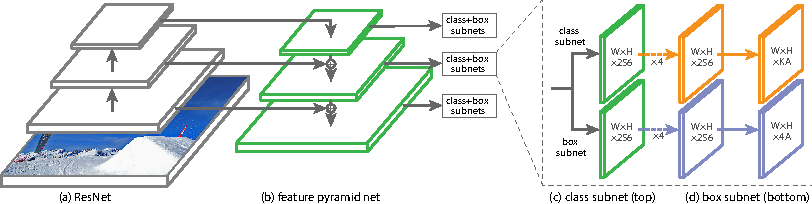
\includegraphics[page=1,width=\linewidth]{images/retinanet.pdf}
    \caption{RetinaNet architecture overview \cite{lin2018focalloss}}
    \label{fig:retinanet}
\end{figure}


\subsubsection{Architecture}
A convolutional backbone (e.g., ResNet) feeds a feature pyramid $\{P_\ell\}$ (typically $P_3$--$P_7$). 
At each pyramid level $\ell$ with spatial size $H_\ell \times W_\ell$, and stride $s_\ell$, a set of $A$ anchors per location is tiled. 
Two subnetworks are applied at each level of the pyramid, producing per-anchor outputs:
\begin{itemize}
    \item \emph{Classification head:} a small CNN produces per-class logits $\hat{z}_{\ell,ij,a,c}$, using independent sigmoids (no softmax) over $c \in \{1,\dots,K\}$.
    \item \emph{Regression head:} a parallel CNN predicts box deltas $\hat{t}_{\ell,ij,a}=(\hat{t}_x,\hat{t}_y,\hat{t}_w,\hat{t}_h)$.
\end{itemize}

Once we obtain the structured outputs from the network, we apply the post-processing steps discussed 
in Section~\ref{sec:anchor_based_detectors} to discard redundant detections.

\paragraph{Focal Loss.}

As previously mentioned, RetinaNet introduced the \emph{focal loss} to address the extreme class imbalance in dense predictions.
It essentially down-weights easy to classify examples and focuses training on hard negatives (Figure~\ref{fig:focal-loss}), which is particularly useful in medical imaging where the background class can dominate the training set. To do so it adds a modulating factor $(1-p_t)^\gamma$ to the cross-entropy loss, with a focus parameter $\gamma$. The focal loss is hence defined as follows:

$$
\mathrm{FL}(p_t) = -\,\alpha\,(1-p_t)^{\gamma}\,\log(p_t),
$$
with typical $\alpha{=}0.25$, $\gamma{=}2$.\\
\begin{figure}[h]
    \centering
    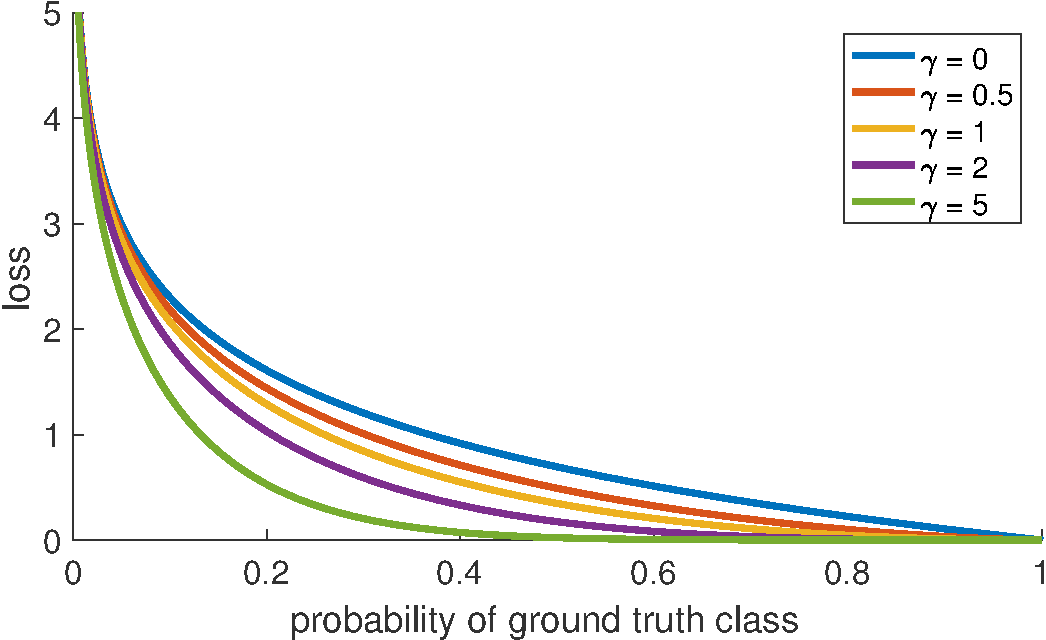
\includegraphics[width=0.55\linewidth]{images/focal-loss.pdf}
    \caption{Focal loss at different $\gamma$ values \cite{lin2018focalloss}. When $\gamma=0$, it is equivalent to cross-entropy loss. As $\gamma$ increases, the loss focuses more on hard examples, down-weighting easy ones.}
    \label{fig:focal-loss}
\end{figure}


\section{Faster R-CNN}
% two-stage anchor-based architecture, the most common one and the one that is used in most of the literature.
% Describe its components, RPN, RoI pooling etc., it is the culmination of the R-CNN family of architecutres.
% f

Faster R-CNN is a two-stage, anchor-based detector that couples a Region Proposal Network (RPN) with a per-region classifier and regressor~\cite{ren2016fasterrcnn}. A shared backbone (we consider one using FPN) feeds both stages.

\begin{figure}[h]
    \centering
    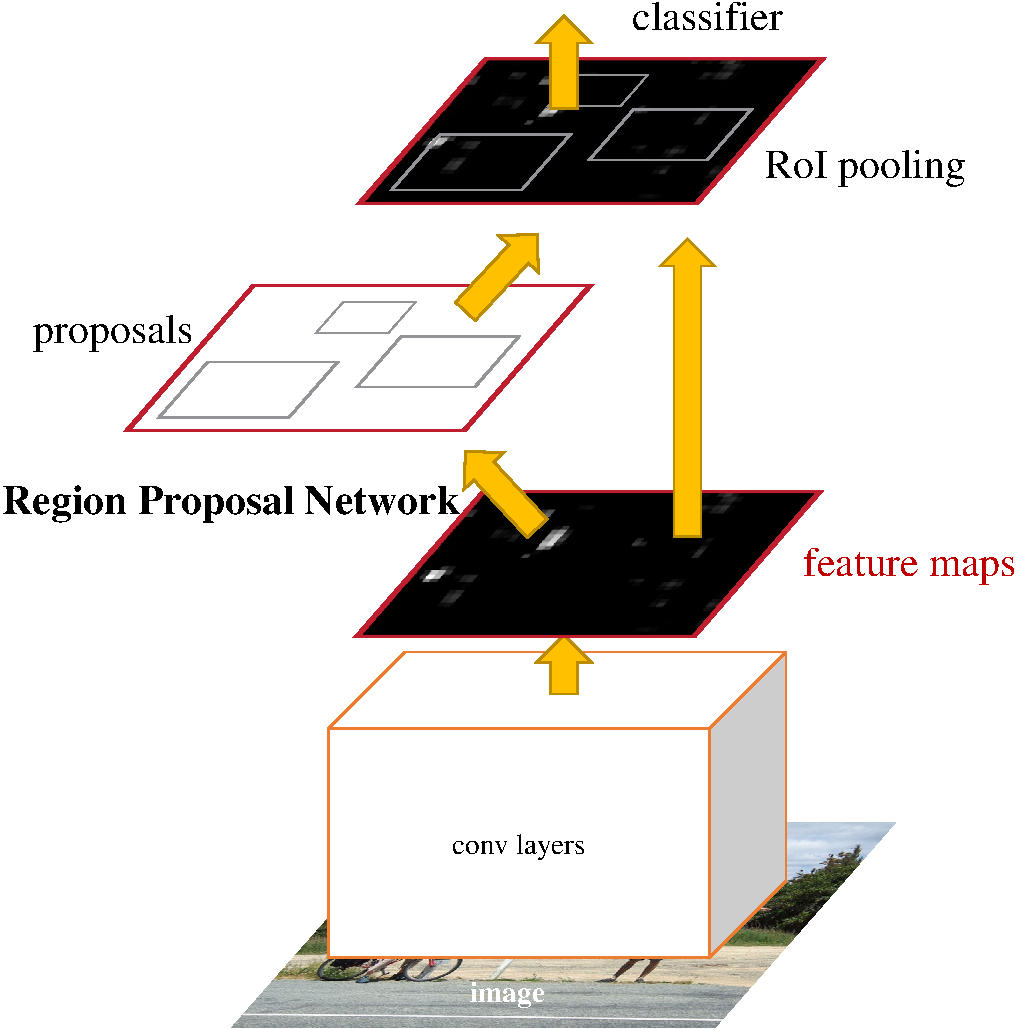
\includegraphics[width=0.6\linewidth]{images/fasterrcnn.pdf}
    \caption{Faster RCNN architecture overview \cite{ren2016fasterrcnn}}
    \label{fig:fasterrcnn}
\end{figure}


\subsubsection{Region Proposal Network (RPN).}
At each feature-map location and for $A$ anchors $a_k=(x_a,y_a,w_a,h_a)$, the RPN predicts:
\begin{itemize}
    \item objectness logits $\hat{o}_k$ (binary);
    \item box deltas $\hat{t}_k=(\hat{t}_x,\hat{t}_y,\hat{t}_w,\hat{t}_h)$.
\end{itemize}
At this stage we do not have any class information, but rather we unify all classes into a single \emph{object} against a \emph{background} class, hence the binary classification. We call \emph{objectness} the probability that an anchor contains an object, regardless of its initial class. Such probability is typically obtained by applying a sigmoid activation to the logits $\hat{o}_k$.\\
Anchors are assigned to ground-truth boxes by IoU thresholds: positives $\mathcal{A}^+$, negatives $\mathcal{A}^-$, ignored $\mathcal{A}^0$. Positives receive class $1$ and regression targets $t_k$ (standard parameterization),
$$
t_x=\frac{x^\ast-x_a}{w_a},\quad
t_y=\frac{y^\ast-y_a}{h_a},\quad
t_w=\log\frac{w^\ast}{w_a},\quad
t_h=\log\frac{h^\ast}{h_a}.
$$

At the end of the RPN, we filter the proposals by objectness score $\hat{o}_k$ and apply non-maximum suppression (NMS) to obtain a sparse set of proposals $\mathcal{P}$, which are then passed to the second stage.\\

We notice how the RPN is a fully convolutional network, therefore the size of input has not to be fixed, although it will increase the number of anchors and thus the computational cost.

\paragraph{Second-stage head.}
The second stage process starts with RoIAlign, a procedure that pools features from the shared backbone for each proposal into a fixed-size tensor $F_j$ (e.g., $7{\times}7{\times}C$) without quantization errors \cite{he2018maskrcnn}. This is done by bilinear interpolation of the feature maps at the proposal locations, which avoids the quantization issues that arise with max pooling, that was a common issue in the original R-CNN architectures using RoIPooling instead.

A per-RoI head predicts:
\begin{itemize}
    \item class logits $\hat{z}_{j,c}$ for $c\in\{1,\dots,K\}$ (softmax over $K{+}1$ including background);
    \item refined box deltas $\hat{u}_{j,c}$ (class-specific) or $\hat{u}_j$ (class-agnostic).
\end{itemize}
With labels $(y_j^\ast, u_j^\ast)$ from matching $p_j$ to ground truth, the loss is
$$
\mathcal{L}_{\text{RoI}}
=\frac{1}{N_{\text{roi}}}\sum_{j}\ell_{\text{ce}}(\hat{z}_{j},y_j^\ast)
+\lambda_{\text{roi}}\frac{1}{N_{\text{pos}}}\sum_{j\in\mathcal{P}^+}\ell_{\text{reg}}(\hat{u}_{j,(y_j^\ast)},u_j^\ast),
$$
where regression applies only to positives $\mathcal{P}^+$.\\

Training of Faster R-CNN is performed end-to-end, with both the RPN and the second-stage detection head sharing the same backbone features. To keep the optimization stable, a sampling strategy is used at both stages to balance the large number of negative examples against the relatively few positives: mini-batches are constructed with a fixed foreground-background ratio for anchors in the RPN and for RoIs in the second stage. The assignment of positives and negatives relies on IoU thresholds -- for the RPN, anchors above a high threshold are treated as positives and those below a low threshold as negatives, while intermediate cases may be ignored; for the RoI head, proposals with sufficiently high IoU to a ground-truth box are considered foreground, and the rest background. During backpropagation, gradients propagate through the RoIAlign operation and further into the shared backbone, but not through the non-differentiable proposal selection and NMS steps, which are treated as fixed post-processing operations. Instead we backpropagate through the pre-NMS detections, with analogous loss functions as the ones used in the RoI heads that uses the notion of objectness and anchor's coordinates, allowing the model to learn to produce better proposals and detections.


% \subsection{DETR}
% a one-stage anchor-free architecture, the first to introduce the transformer architecture in object detection, it is a fully end-to-end architecture that does not rely on anchors or region proposals, but rather directly predicts the bounding boxes and class labels in a single pass. Unfortunately, it is not suitable for our use case due to its large needs of data.

\section{Evaluation Metrics: Average Precision and Average Recall}
\label{sec:eval_metrics}
 
To quantitatively evaluate the performance of an object detection model, we rely on the standardized metrics established by the COCO challenge: Average Precision (AP) and Average Recall (AR). While the concepts of precision and recall are simple in classification tasks, their application to object detection is more nuanced.

The core challenge lies in defining what constitutes a True Positive (TP), a False Positive (FP), and a False Negative (FN). A simple binary match is insufficient, as a prediction must be evaluated on both its class label and its spatial accuracy. Furthermore, unlike in classification, the concept of a True Negative is generally considered ill-defined in object detection, as it would represent the infinite number of correctly non-detected objects in the background.

\subsubsection{The Matching Procedure}
To formalize the definition of TP, FP, and FN, we must first define a matching procedure. Given an input image $I$, the model produces a structured output $O$ containing a set of predicted bounding boxes, $\mathcal{B}_{pred}$. This is compared against the structured ground truth label, $\ell$, which contains the set of ground truth boxes, $\mathcal{B}_{gt}$.

The matching procedure, $\mathcal{M}_{\alpha}$, links predicted boxes to ground truth boxes based on a specific Intersection over Union (IoU) threshold, $\alpha$. This procedure, detailed in Algorithm \ref{alg:matching-procedure}, allows us to categorize each prediction.
 
\begin{algorithm}
    \caption{Matching Procedure for Object Detection}
    \label{alg:matching-procedure}
    \DontPrintSemicolon
    \SetAlgoLined
    \setstretch{1.2}

    \SetKwInOut{Input}{Input}
    \SetKwInOut{Output}{Output}
    \Input{
        $\mathcal{B}_{pred}$ (predicted boxes), 
        $\mathcal{B}_{gt}$ (ground truth boxes), 
        $\alpha$ (IoU threshold)
    }
    \Output{Counts for TP, FP, FN}

    \BlankLine
    
    % \tcc{Initialization}
    Initialize each $b_{gt}$ in $\mathcal{B}_{gt}$ as \texttt{unmatched}\;
    Sort $\mathcal{B}_{pred}$ in descending order of confidence scores\;
    TP $\gets 0$, FP $\gets 0$, FN $\gets 0$\;
    
    \BlankLine
    
    \ForAll(){$b_{pred}$ \textup{in sorted} $\mathcal{B}_{pred}$}{
        Find $best\_b_{gt}$ such that:\;
        \quad - $best\_b_{gt}$ is the box in $\mathcal{B}_{gt}$ with the highest IoU with $b_{pred}$\;
        \quad - $best\_b_{gt}$ is currently \texttt{unmatched}\;
        
        \BlankLine
        
        \If{$best\_b_{gt}$ \textup{exists and IoU(}$b_{pred}, best\_b_{gt}$\textup{)} $> \alpha$}{
            TP $\gets$ TP + 1\;
            Mark $best\_b_{gt}$ as \texttt{matched}\;
        }
        \Else{
            FP $\gets$ FP + 1\;
        }
    }
    
    \BlankLine
    
    \ForAll(){\textup{unmatched} $b_{gt}$ \textup{in} $\mathcal{B}_{gt}$}{
        FN $\gets$ FN + 1\;
    }

    \Return{TP, FP, FN}\;

\end{algorithm}With this procedure, for any given IoU threshold $\alpha$, we can now use the standard definitions of Precision and Recall:
\begin{equation}
    \text{Precision}(\alpha) = \frac{\text{TP}(\alpha)}{\text{TP}(\alpha) + \text{FP}(\alpha)}, \quad \text{Recall}(\alpha) = \frac{\text{TP}(\alpha)}{\text{TP}(\alpha) + \text{FN}(\alpha)}
\end{equation}

\subsubsection{Defining AP and AR}
Before stating the definitions of AP and AR, it is important to note that these will slightly differ from the original COCO definitions, as in some cases COCO has not stated them formally, introducing some ambiguity.

By varying the confidence score threshold for the predictions, we can trace a Precision-Recall (PR) curve for a fixed IoU threshold $\alpha$. Let this curve be described by the function $p(\alpha, r)$, where $r$ is the recall level.

The Average Precision (AP) at a given IoU threshold $\alpha$ is defined as the area under this PR curve:
\begin{equation}
    \text{AP}@\alpha = \int_{0}^{1} p(\alpha, r) \,dr
\end{equation}

The Average Recall (AR) is defined differently. It is the maximum recall achieved given a fixed number of top-scoring detections per image, $k$. Let $r(\alpha, k)$ be the recall as a function of the IoU threshold and the number of predictions $k$. The AR is then:
\begin{equation}
    \text{AR}@\alpha = \max_{k \in \{1, 10, 100\}} r(\alpha, k)
\end{equation}

To provide a single, comprehensive metric for model performance, we can compute the AP and AR by averaging the values over a range of IoU thresholds. Let $S = \{0.05, 0.10, \dots, 0.95\}$. The final metrics are:
\begin{equation}
    \text{AP}@S = \frac{1}{|S|} \sum_{\alpha \in S} \text{AP}@\alpha
\end{equation}
\begin{equation}
    \text{AR}@S = \frac{1}{|S|} \sum_{\alpha \in S} \text{AR}@\alpha
\end{equation}
An alternative and common notation for AP@S is AP@5:95. This multi-threshold evaluation ensures that the metric rewards models that are accurate across a wide spectrum of localization strictness.

Finally, in order to take into consideration multiple classes, we can define the mean Average Precision (mAP) and mean Average Recall (mAR) as follows:
\begin{equation}
    \text{mAP}@\alpha = \frac{1}{K} \sum_{k=1}^{K} \text{AP}_k@\alpha
\end{equation}
\begin{equation}
    \text{mAR}@\alpha = \frac{1}{K} \sum_{k=1}^{K} \text{AR}_k@\alpha
\end{equation}
where $K$ is the number of classes, and $\text{AP}_k$ and $\text{AR}_k$ are the AP and AR for class $k$, respectively. A similar definition can be applied to $\mathrm{mAP}@S$ and $\mathrm{mAR}@S$.


\section{XAI for Deep Learning in Computer Vision Tasks}
The impressive performance of deep learning models in numerous fields -- including medical imaging -- is often accompanied by a significant challenge: their ``black box'' nature \cite{chaddad2023survey, singh2025beyond}. These models, composed of millions of parameters, learn complex hierarchical features from data, but their decision-making processes are not inherently transparent \cite{moradi2024model}. In high-stakes fields like clinical diagnostics, where a model's conclusion could influence patient care, this lack of transparency is a major barrier to adoption and trust \cite{chaddad2023survey,glikson2020human}. Clinicians and regulatory bodies require assurance that a model is not only accurate but also bases its predictions on clinically relevant features, rather than confounding artifacts in the data \cite{kingma2017adam}.
Explainable AI (XAI) is a field dedicated to developing methods that render these complex models more understandable to humans.\cite{chaddad2023survey,kinger2024review}. The goal is to provide insights into the model's decision-making process, making it a ``gray-box'' model, which, while not fully transparent, offers an important insight into its reasoning. For computer vision tasks, one of the most intuitive and powerful families of XAI techniques is Class Activation Maps (CAM) \cite{minh2023overview}.

%Quick introduction of explainability in deep learning, highlighting how models are essentially black boxes and the need to understand, although partially, their inner workings. This need is even more pronounced in the medical field, where explainability is a requirement for clinical acceptance and regulatory compliance. Highlight how explainability methods, especially the ones that we are going to cover, are desinged to provide \emph{insights} into the model's decision-making process, it does not make it fully explainable, but rather makes it a gray-box model, which is still better than a black box.
% Trainsition to CAMs for computer vision tasks

\subsection{Class Activation Maps (CAM)}
Class Activation Maps, or CAMs, are visualization techniques that produce heat\-maps to highlight the discriminative regions in an image that a model used to make a specific prediction \cite{minh2023overview}. In the context of lung nodule detection, a CAM would highlight the pixels within a CT scan slice that were most influential in the model's decision to identify a nodule.
It is important to note that the most influential regions highlighted by CAMs are not necessarily the same as the regions that contain the object of interest. For instance, a model might focus on contextual cues or surrounding tissue patterns that correlate with the presence of a nodule, or use spurious correlations that do not directly correspond to the object itself. Therefore, while CAMs provide valuable insights into the model's reasoning, they should be interpreted with caution and in conjunction with domain knowledge.

The original CAM method required a specific network architecture containing a Global Average Pooling (GAP) layer before the final output layer \cite{zhou2016learning}. It works by extracting the feature maps from the final convolutional layer and weighting each map by the weights connecting it to the output neuron for the class of interest. The resulting weighted sum of feature maps produces a heatmap localized on the features most relevant to that class.

A more flexible and widely used extension is Gradient-weighted Class Activation Mapping (Grad-CAM) \cite{selvaraju2019gradcam}. Grad-CAM generalizes the CAM approach by removing the need for a specific architecture. It calculates the importance of each neuron in the final convolutional layer by using the gradient of the class score with respect to the feature maps of that layer.
Regions with a large gradient are those where a change in pixel intensity would have a significant impact on the class score, indicating their importance. This gradient-based approach allows Grad-CAM to be applied to a wide variety of CNN architectures without modification.

Several other CAM variants have been proposed to address limitations of Grad-CAM, such as the inclusion of other layers in the calculations to improve resolution and localization, its reliance on gradients -- which can be noisy and unstable -- or simply how the gradients are handled. 
Notable gradient-free methods include Score-CAM \cite{wang2020score}, which uses the model's output scores to weight the feature maps instead of gradients; Eigen-CAM \cite{muhammad2020eigen}, which employs principal component analysis to identify the most significant features.

% What are CAMs, how they work, and their (usual) limitations. Describe GradCAM as a gradient-based method and then explain why it is problematic for object detection tasks due to their sensitivity to the structured outputs and the non-differentiable post-processing steps. 

\subsection{CAM's Limitations for Object Detection}
While methods like Grad-CAM are highly effective for classification tasks, they cannot be directly applied to object detection models without prior modifications. These limitations arise from the fundamental differences between the two tasks, but mostly regarding the structural difference of the model's output and the post-processing operations involved.

The first significant hurdle is the structured output problem. A classification model produces a single scalar score for a given class (e.g., the logit or probability that an image contains a "nodule"). This single, well-defined score serves as a clear target for computing gradients. An object detection model, in contrast, produces a variable-length list of predictions. Each prediction is a composite structure containing: a bounding box with spatial coordinates (x, y, width, height), a class label (e.g., "nodule"), and a confidence score.

This raises a critical question: if the model detects multiple potential nodules, which prediction's score should be backpropagated to generate the explanation? Choosing the highest-scoring box might ignore other valid detections, while averaging scores could dilute the explanation. This ambiguity complicates the fundamental requirement of having a single, differentiable target score.

The second, and more critical, limitation is the non-differentiability of the detection pipeline. Object detection models rely on a crucial post-processing step known as Non-Maximum Suppression (NMS) discussed in Section~\ref{sec:anchor_based_detectors}.
This algorithmic filtering is not a differentiable operation. A minuscule change in a feature map within the network could lead to a slight change in a box's confidence score. This seemingly insignificant change could alter the ranking of boxes, causing NMS to discard a prediction it would have otherwise kept, or vice versa. This creates sharp discontinuities in the end-to-end function from the model's feature maps to its final output. Consequently, the gradient becomes unstable or, at these points of discontinuity, completely undefined.

For an explanation method to be considered faithful, it must be stable; small, imperceptible changes to the input should not cause wild fluctuations in the explanation. The unstable gradients caused by NMS mean that a gradient-based explanation -- such as Grad-CAM -- for an object detector can be unreliable. Two nearly identical CT slices might produce drastically different heatmaps, undermining the very trust the explanation is meant to build. These challenges motivate the need for an alternative approach, leading to the adaptation of gradient-free CAM methods for the object detection task.

\subsection{Adaptations for Object Detection}
Given the inherent limitations of gradient-based methods in the context of object detection, our work turns to gradient-free CAM techniques. These methods do not rely on backpropagation and are therefore robust against the challenges posed by non-differentiable operations like NMS.
Among these, Eigen-CAM is the most straightforward to apply. Its methodology generates explanations by performing a Principal Component Analysis (PCA) on the activation maps of a target layer. Since this process is entirely self-contained within the feature maps and does not depend on the model's final output, it works "out-of-the-box" for object detection architectures without any modification.
However, more sophisticated methods like Score-CAM and its variants, which are class-discriminative, require significant adaptation to handle the structured outputs of an object detector.

\subsubsection{Adapting Score-CAM}

To understand the necessary adaptations, we must first revisit the core mechanism of Score-CAM in its original classification context. The final Score-CAM explanation, $L^{c}_{\text{Score-CAM}}$, for a class $c$ is formally defined as the ReLU-clipped, weighted linear combination of the activation maps $A^{k}_{\ell}$ from a target convolutional layer $\ell$
\begin{equation}
    L^{c}_{\text{Score-CAM}} = \mathrm{ReLU}\left( \sum_{k} \alpha^{c}_{k} A^{k}_{\ell} \right)
    \label{eq:scorecam}
\end{equation}

The critical component here is the weight $\alpha^{c}_{k}$, which represents the importance of the \textit{k}-th activation map for class \textit{c}. Score-CAM calculates this weight using a metric called the Channel-wise Increase in Confidence (CIC). The CIC for an activation map $A^{k}_{\ell}$ is given by:
\begin{equation}
    \alpha_k^c = \text{CIC}\left(A^{k}_{\ell}\right) = f\left(X \circ H^{k}_{\ell}\right) - f(X_{b})
    \label{eq:cic}
\end{equation}

Where:
\begin{itemize}
    \item $f(\cdot)$ is the forward pass of the model, which outputs a confidence score for the target class.
    \item $X$ is the input image tensor.
    \item $f(X_{b})$ is the baseline score from the original, unperturbed image.
    \item $\circ$ denotes the element-wise product.
    \item $H^{k}_{\ell}$ is a mask generated from the activation map $A^{k}_{\ell}$ by upsampling it to the input image size and normalizing its values to the range $[0, 1]$. This is defined as:
    \begin{equation}
        H^{k}_{\ell} = s\left(\text{Up}\left(A^{k}_{\ell}\right)\right)
        \label{eq:mask_generation}
    \end{equation}
    Here, $\text{Up}(\cdot)$ is the upsampling operation and $s(\cdot)$ is the normalization function.
\end{itemize}

This mathematical framework fundamentally breaks down when applied to an object detector. The model's forward pass, $f(\cdot)$, does not return a single scalar confidence score. Instead, $f(X \circ H^{k}_{\ell})$ and $f(X_{b})$ produce structured outputs: variable-length lists of detections, each with its own bounding box, class label, and score. Consequently, the subtraction operation in the CIC formula (Equation \ref{eq:cic}) is mathematically undefined. It is not arithmetically possible to subtract one set of detections from another.

This necessitates a new way to measure the ``increase in confidence'' or, more accurately, the similarity between two sets of structured predictions.

Our solution is to replace the undefined subtraction with a custom scoring function, implemented as \texttt{FasterRCNNBoxScoreTarget}. This function effectively quantifies how well the model's output from a perturbed image aligns with its original, baseline output. It transforms the comparison of two complex outputs into a single, scalar similarity score, which can then be used as the weight $\alpha^{c}_{k}$ in the Score-CAM algorithm.

The \texttt{FasterRCNNBoxScoreTarget} function operates as described in Algorithm \ref{alg:box-score-target}. It takes as input the original detections $D_{orig}$ from the unperturbed image and the new detections $D_{new}$ from the perturbed image. The function computes a similarity score by iterating over each bounding box in the original detections and finding the best matching box in the new detections based on Intersection over Union (IoU) and class label agreement.
The final output of the function is the sum of these individual scores, resulting in a single scalar value. This value represents the overall similarity between the original and perturbed detections and serves as a direct replacement for the CIC score in the Score-CAM framework.


\begin{algorithm}
    \caption{FasterRCNNBoxScoreTarget: Similarity Scoring for Object Detection Outputs}
    \label{alg:box-score-target}
    \DontPrintSemicolon
    \SetAlgoLined
    \setstretch{1.2}

    \SetKwInOut{Input}{Input}
    \SetKwInOut{Output}{Output}
    
    \Input{
        $D_{orig}$: original detections \{boxes, labels, scores\}\;
        $D_{new}$: new detections from perturbed image \{boxes, labels, scores\}\;
        $T_{iou}$: IoU threshold for matching
    }
    \Output{A scalar similarity score}

    \SetKwData{totalScore}{totalScore}
    \SetKwData{ious}{ious}
    \SetKwData{bestIoU}{bestIoU}
    \SetKwData{matchIndex}{matchIndex}
    \SetKwData{boxScore}{boxScore}

    \BlankLine

    $\totalScore \gets 0.0$\;
    
    \ForAll(){(box$_{orig}$, label$_{orig}$, score$_{orig}$) \textup{in} $D_{orig}$}{
        \If{$D_{new}$ \textup{is not empty}}{
            % \tcc{Find the best matching new detection}
            $\ious \gets$ ComputeIoU(box$_{orig}$, boxes$_{new}$)\;
            $\bestIoU, \matchIndex \gets$ FindMaxWithValueAndIndex($\ious$)\;
            
            \BlankLine
            % \tcc{Check if the match is valid (sufficient overlap and same class)}
            label$_{new} \gets$ labels$_{new}$[$\matchIndex$]\;
            \If{$(\bestIoU > T_{iou})$ \textup{and} $(label_{orig} = label_{new})$}{
                % \tcc{Calculate score based on IoU and confidence similarity}
                score$_{new} \gets$ scores$_{new}$[$\matchIndex$]\;
                $\boxScore \gets \bestIoU \times (1 - (score_{new} - score_{orig})^2)$\;
                $\totalScore \gets \totalScore + \boxScore$\;
            }
        }
    }
    
    \Return{$\totalScore$}\;
\end{algorithm}

\subsubsection{Adapting Smoothed Score-CAM (SS-CAM)}
\label{subsubsec:adapting_sscam}

Smoothed Score-CAM (SS-CAM) is an extension of Score-CAM designed to produce less noisy and more robust explanations. It achieves this by introducing a small amount of random noise to the activation map masks before they are applied to the input image, repeating this process over $N$ trials, and averaging the resulting scores.

Formally, the weight $\alpha^{c}_{k}$ for each activation map is computed as an average of the CIC scores obtained from stochastically perturbed masks:
\begin{equation}
    \alpha^{c}_{k} = \frac{1}{N} \sum_{i=1}^{N} \text{CIC}\left(f\left(X \circ \left(H^{k}_{l} + D_i\right)\right)\right)
    \label{eq:sscam_weight}
\end{equation}
where $D_i$ is a noise tensor sampled from a distribution, typically a Gaussian $\mathcal{N}(0, \sigma^2)$.

This method naturally inherits the same fundamental challenge as Score-CAM regarding the structured outputs of object detectors. The CIC calculation, and its core subtraction operation, remains mathematically undefined. Therefore, the primary adaptation is identical: we replace the scoring mechanism with the \texttt{FasterRCNNBoxScoreTarget} algorithm (as defined in Algorithm \ref{alg:box-score-target}) to compute a scalar similarity score for each of the $N$ noisy forward passes.

However, a second, more subtle adaptation was required during implementation, which is unique to the SS-CAM methodology. The original SS-CAM papers often assume input images with pixel values in the integer range $[0, 255]$. In medical imaging pipelines, it is standard practice to normalize images to a floating-point range, such as $[0, 1]$. When using such normalized inputs, the magnitude of the noise proposed by the original SS-CAM method can easily overwhelm the signal from the activation map mask itself, leading to meaningless scores and unstable explanations.

To address this, we introduce a minor but critical modification: the Gaussian noise is scaled down significantly before being added to the mask. This is implemented in our code with the operation \texttt{noise.div\_(20.)}. This adjustment ensures that the noise acts as a gentle perturbation, smoothing the explanation space around the original prediction as intended, rather than dominating the input and corrupting the measurement.
